\documentclass[a4paper,11pt, twoside]{article}

\usepackage[a4paper,top=3cm,bottom=3.5cm,left=2.5cm,right=2.5cm]{geometry}
\usepackage{graphicx}
\usepackage[utf8x]{inputenc}
\usepackage[italian]{babel}
\usepackage{fancyhdr}
\usepackage{amssymb}
\usepackage{makeidx}
\usepackage{eurosym}
\usepackage{hyperref}
\usepackage{varioref}
\usepackage{xmpincl}
\usepackage{ccicons}
\usepackage{subfigure}
\usepackage{amsmath}

\usepackage{amsthm}

\theoremstyle{definition}
\newtheorem{defn}{Definizione}[section]

\title{Appunti di Progettazione Hardware 2}
\author{Matteo Gianello}
\date{\today}

\pdfinfo{%
  /Title    (Appunti di Progettazione Hardware 2)
  /Author   (Matteo Gianello)
  /Creator  (Matteo Gianello)
  /Producer ()
  /Subject  ()
  /Keywords (Progettazione Hardware 2 Ferrandi IngInf Polimi)
}
\makeindex
\includexmp{licenza}

\begin{document}
\maketitle
\thispagestyle{empty}
\vspace{5cm}
\begin{center}
Quest'opera è stata rilasciata con licenza Creative Commons Attribuzione - Non commerciale - Condividi allo stesso modo 3.0 Unported. Per leggere una copia della licenza visita il sito web \url{http://creativecommons.org/licenses/by-nc-sa/3.0/deed.it} \ccbyncsa.
\end{center}
\newpage
\setcounter{page}{1}
\tableofcontents
\newpage

\pagestyle{plain}

\label{capitolo1}
\section{Progettazione a basso consumo di potenza}
Nel corso degli anni ci si è spostati verso la progettazione di sistemi hardware che consumassero sempre meno. Le motivazioni che hanno portato a questa evoluzione sono molteplici e di diversa natura; alcune di queste sono:
\begin{description}
\item[Tecnologiche:] l'aumento della frequenza e dei transistor presenti nel circuito obbligano ad un minor consumo di energia
\item[Commerciali:] la diffusione di dispositivi portatili che richiedono alte prestazioni e un basso consumo energetico
\item[Economiche:] ridurre il costo del \emph{packaging} del comparto batterie
\end{description}
La diffusione di dispositivi portatili ha portato ad avere un \emph{trade-off} tra le performance ed il consumo energetico.\\
Il design a basso consumo e le metodologie di stima del consumo di potenza devono essere valutate ad un diverso livello di astrazione durante tutto il processo di progettazione; i diversi livelli sono
\begin{itemize}
\item System Level
\item Behavioral Level
\item RT (Register Transfer) Level
\item Gate Level
\item Transistor Level
\end{itemize}
L'evoluzione attuale della tecnologia delle batterie è insufficiente rispetto all'evoluzione odierna dei circuiti, infatti, le capacità delle batterie aumentano all'incirca del 10\%-15\% all'anno mentre il consumo dei circuiti aumenta molto più velocemente, questo comporta un gap notevole tra il fabbisogno di potenza dei circuiti e la disponibilità data dai pacchi batterie.\\
Ad oggi la tecnologia più utilizzata per la realizzazione di circuiti digitali è quella \textbf{CMOS} in quanto la velocità di switching è notevole ed il consumo di corrente è intrinsecamente basso.
Il consumo di potenza nei CMOS è dato da 
$$P=P_{switching}+P_{short-circuit}+P_{leakage}$$
Dove $P_{switching}$ è la potenza necessaria per caricare e scaricare il condensatore durante il cambio di contesto del transistor $P_{short-circuit}$ è la corrente che va da $V_{dd}$ a $GND$ durante la transizione di uscita ed infine $P_{leakage}$ è la componente data dalla corrente di leakage.\\
La parte $P_{switching}$ è la parte predominante della dissipazione di potenza e l'obiettivo dei progettisti è quello di minimizzare questo fattore durante la fase di design del sistema. Per quanto riguarda, invece, $P_{short-circuit}$ e $P_{leakage}$ per minimizzarli occorre agire a livello tecnologico e non risulta essere una cosa semplice.\\
\begin{figure}
\centering
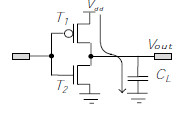
\includegraphics[width=10cm]{img/vddoutput.png}
\label{fig:vddoutput}
\caption{Transizione $0 \rightarrow V_{dd}$}
\end{figure}
\section{Modelling}\label{capitolo2}
Al giorno d'oggi esistono una serie di computer il cui scopo principale non è quello di gestire informazioni, bensì quello di interagire con i sistemi fisici, questo tipo di computer è chiamato \emph{sistema embedded}, alcuni esempi di sistemi embedded sono:
\begin{itemize}
\item controlli automotive
\item avionica
\item dispositivi medici
\item controlli industriali
\item dispositivi di gestione e conservazione dell'energia
\end{itemize}
Un sistema embedded è un sistema di calcolo ma non principalmente un computer integrato con un insieme di processi fisici tramite sensori, attuatori ecc. il quale deve essere \emph{reattivo} ovvero deve rispettare dei vincoli temporali, è \emph{eterogeneo} in quanto formato da componenti hardware, software, componenti di rete; ed infine è \emph{distribuito} e \emph{concorrente}.
Un esempio di questo tipo di sistema lo troviamo sulle auto moderne dove sono presenti fino ad 80 computer denominate ECU (\emph{electronic control units}), esse variano dal controllo del motore e della trasmissione fino al controllo audio e di climatizzazione ma anche i display e la strumentazione di bordo. Sono presenti più di 100 milioni di linee di codice e tutti i sistemi sono collegati tramite CAN bus e oltre 2 km di cavi. Tale parte incide sempre più sul costo di una automobile.\\
Una parte molto importante di un sistema embedded è il software che viene eseguito su di esso in quanto deve sfruttare risorse limitate mantenendo performance elevate. Ad esempio la corretta esecuzione di un programma in \emph{C}, \emph{C\#}, Java etc. non tiene conto del tempo impiegato per l'esecuzione e ogni nostra astrazione è fondata su questa premessa; il tempo di esecuzione di un programma non è un fattore certo e ripetibile a meno che non prendiamo in considerazione una granularità molto grossa per l'analisi. Alcuni esempi che sfruttano l'irrilevanza del tempo nei sistemi normali sono il \emph{garbage collector}, la \emph{just-in-time} compilation, il \emph{power managment} e molti altri.\\
In un sistema embedded invece bisogna tener conto delle risorse limitate come la poca memoria e la dimensione della parola più corta e la frequenza di clock bassa. Per tener conto di queste limitazione ci si concentra sull'efficenza scrivendo software a basso livello (C, Assembly), si evitano sistemi operativi con molte funzionalità, si utilizzano architetture specializzate (DSP, Network) si utilizzano sistemi di interconnessione specializzati. Inoltre i sistemi embedded si differenziano da quelli \emph{general-purpose} in quanto devono rispettare dei vincoli temporali ("il più velocemente possibile" non è abbastanza), la concorrenza è intrinseca, le specifiche dei processori sono specializzate per rispettare i vincoli temporari supportare le operazioni più comuni e utilizzare specifici tipi di dati ed infine i programmi devono poter essere eseguiti \emph{per sempre} il reboot del sistema non è accettabile.\\
Il concetto di \emph{real-time} è più complicato del concetto del \emph{"prima possibile"}, in realtà esso indica dei limiti temporali che non possono essere valicati, oggi i programmatori di sistemi embedded costruiscono il sistema e successivamente lo testano per il timing. Un meccanismo basato sui modelli cerca di specificare il comportamento dinamico inclusi i vincoli temporari per poi \emph{"compilare"} un'implementazione che rispecchi le specifiche.\\
In molti casi i sistemi operativi real-time (\emph{RTOS}) sono utilizzati in maniere inappropriate, senza considerare particolari principi o funzionalità. Gli sviluppatori modificano le priorità fino a quando il prototipo non soddisfa i test. Tuttavia il sistema che ne risulta è fragile e un piccolo cambiamento nelle condizioni di operatività può causare grandi cambiamenti nel comportamento del sistema.\\
L'astrazione ha lo scopo di nascondere i dettagli dell'implementazione in modo da fornire una piattaforma sulla quale progettare. Un design basato su modelli può essere pensato a diversi livelli come strutturale, funzionale, orientato agli attori, ecc. questo permette uno sviluppo intuitivo del sistema tramite degli artifici che lo imitano. Un esempio è il \emph{modello matematico} il quale rappresenta il sistema tramite un insieme di definizioni e formule matematiche. Creare un modello matematico di tutte le parti di un sistema può portare alla costruzione automatica del sistema come avviene per un compilatore.\\
Esistono diverse tecniche di modello ognuna adatta a rappresentare un aspetto diverso del sistema, ad esempio:
\begin{itemize}
\item \textbf{Macchine a statti:} utile per rappresentare decisioni logiche sequenziali.
\item \textbf{Modelli basati sul flusso dei dati:} utili per esplorare il parallelismo e per il processo dei segnali.
\item \textbf{Modelli ad eventi discreti:} nel quale viene esplicitato il tempo.
\item \textbf{Modelli time-driven:} che studiano eventi periodici e azioni temporali
\end{itemize}
\subsection{Modelli di computazione}
Un \emph{modello di computazione} è un assegnamento di semantica, ovvero di significato, alla sintassi definita dal modello. Il \emph{MoC} definisce le regole per eseguire il modello, queste regole deteminano come gli attori intervengono sulla computazione, aggiornano i loro stati interni e interagiscono con l'esterno. Infine il modello di computazione definisce come diversi componenti comunicano tra loro.\\
Prendiamo in considerazione l'esempio di \figurename\,\ref{fig:parkschema} nel quale viene mostrato un contatore per le auto che entrano ed escono da un parcheggio.
\begin{figure}
\centering
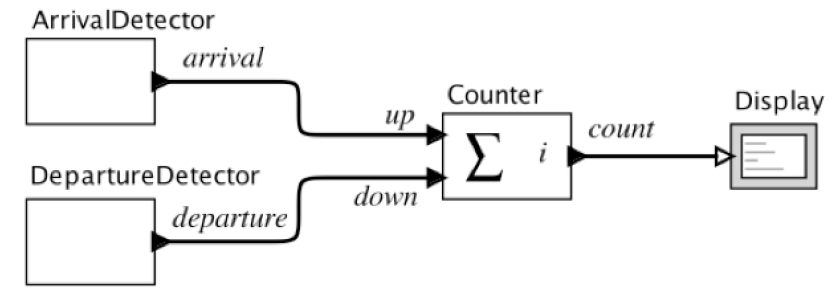
\includegraphics[scale=0.4]{img/parkschema.png}
\caption{Schema di un contatore per un parcheggio}\label{fig:parkschema}
\end{figure}
In questo caso vediamo che il sistema è composto da:
\begin{description}
\item[Segnali puri:] $up, \ down : \mathbb{R}\rightarrow\{absent,present\}$
\item[Attori discreti:]\emph{Contatore}:$(\mathbb{R}\rightarrow\{absent,present\})^P \rightarrow(\mathbb{R}\rightarrow\{absent\}\cup \mathbb{N})\_P=\{up,down\}$
\end{description}
Definiamo \emph{reazione} il fenomeno per cui per qualsiasi $t\in\mathbb{R}$ dove $up(t)\neq absent$ o  $down(t)\neq absent$ il \emph{Contatore} reagisce ovvero produce un output in $\mathbb{N}$ e modifica il suo stato interno.
Per ogni $t\in\mathbb{R}$ la porta \emph{p} ha una valorizzazione ovvero un assegnamento dei valori che per la porta $P=\{up,down\}$ corrisponde all'assegnamento sui due ingressi di uno dei due valori $\{absent, present\}$. Una reazione non è altro che una valorizzazione dell'output, in questo caso $count$ assume uno dei valori nel set $\{absent\}\cup \mathbb{N}$.\\
Un'altra definizione che dobbiamo dare è quella dello \emph{spazio degli stati} che non è altro che l'insieme degli stati in cui si può trovare il nostro contatore. Nel nostro caso il parcheggio ha un numero finito $M$ di posti disponibili perciò lo spazio degli stati per il nostro contatore è
$$State = \{0,1,2,3,\dots,M\}$$
Un modo per rappresentare il comportamento del nostro sistema è quello di utilizzare una \emph{Macchina a Stati Finiti}(\emph{FSM}) come quella di \figurename\,\ref{fig:parkfsm} nella quale possiamo distinguere alcuni tratti caratteristici:
\begin{description}
\item[Guardia:] insieme di valori che indicano i valori che devono essere presenti sugli input affinchè avvenga un cambio di stato, per l'arco che va da \emph{0} a \emph{1} la guardia è:
$$up \wedge \neg down $$ 
\item[Stato iniziale:] è quello indicato da una freccia entrante in questo caso è lo stato indicato da \emph{0}
\item[Valore di uscita:] è il valore che viene prodotto durante un passaggio di stato in questo caso è il valore del contattore, nella macchina a stati finiti è indicato dal valore a destra della \emph{guardia.}
\end{description}
\begin{figure}
\centering
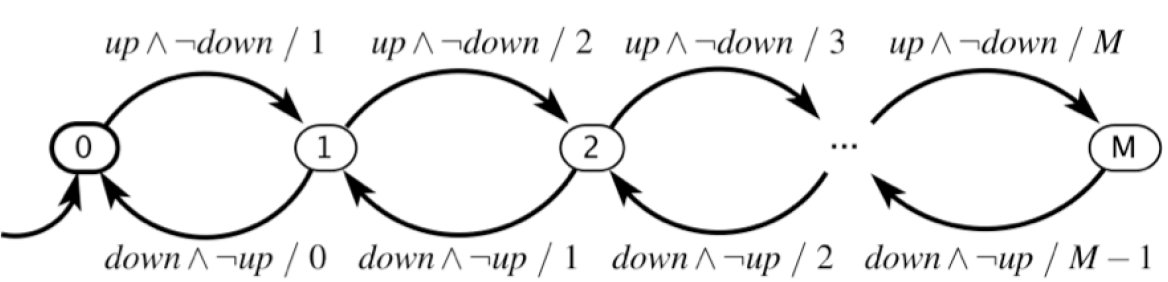
\includegraphics[scale=0.4]{img/parkfsm.png}
\caption{Macchina a stati finiti di un contatore per un parcheggio}\label{fig:parkfsm}
\end{figure}
Per definire una macchina a stati finiti formalmente sono necessari gli \emph{stati}, gli \emph{inputs}, gli \emph{outputs}, gli \emph{update} e lo \emph{stato iniziale}.\\
Una \emph{transizione di default} è una transizione che viene attivato solo quando le transizioni di default non sono attive e nessuna guardia è valutata come vera, un esempio di tale tipo di transizione è mostrata in \figurename\,\ref{fig:defaulttrans}.\\
\begin{figure}
\centering
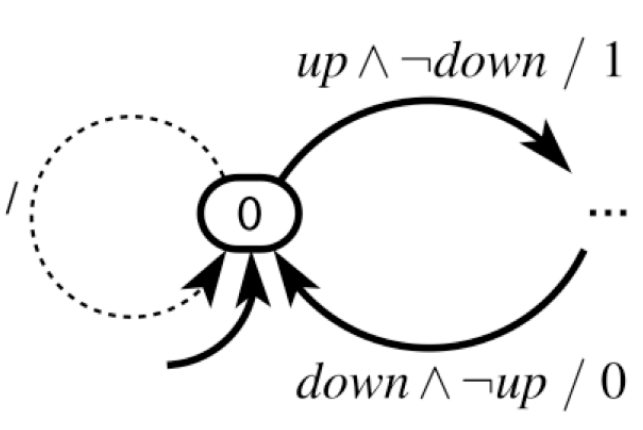
\includegraphics[scale=0.4]{img/defaulttrans.png}
\caption{Esempio di transizione di default}\label{fig:defaulttrans}
\end{figure}
Una transizione \emph{stuttering} è una tranzione di default implicita che viene abilitata in assenza di input e che non produce output. La \emph{ricettività} è una proprietà delle macchine a stati che afferma che per qualsiasi valore in input almeno una transizione è abilitata, le strutture con transizioni di default fanno in modo che le FSM siano ricettive.\\
Il \emph{determinismo} è una proprietà importante delle macchine a stati finite e afferma che in ogni stato per tutti i valori di input esattamente una transizione viene abilitata.\\
Il \emph{comportamento} di una FSM è definito come una sequenza di transizioni non \emph{stuttering}, una \emph{traccia} è un insieme di input, stati e output di un comportamento; un \emph{albero di computazione} è una rappresentazione grafica di tutte le possibile tracce. Tale proprietà fa si che le FSM siano analizzabili formalmente.\\
Il \emph{non determinismo} è la possibilità di avere, in una FSM, due possibili scelte per lo stesso valore di ingresso, un esempio di non determinismo è  mostrato in \figurename\,\ref{fig:nondetfsm}; la funzione di aggiornamento si trasforma in:
$$possibleUpdate : States \times Inputs \rightarrow 2^{States \times Outupts}$$
\begin{figure}
\centering
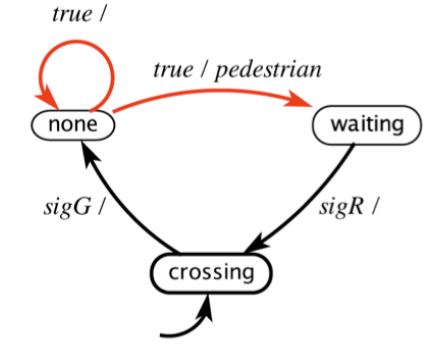
\includegraphics[scale=0.5]{img/nondetfsm.png}
\caption{Esempio di macchina a stati non deterministica}\label{fig:nondetfsm}
\end{figure}
Il non determinismo è molto utile nella fase di modellazione del sistema in quanto permette di modellizzare aspetti ignoti riguardante l'ambiente esterno, nascondere dettagli di una specifica, infine il non determinismo è più compatto da rappresentare.\\
Le macchine a stati finiti permettono di rappresentare un sistema in modo tale che esso sia analizzato matematicamente e manipolato, modellare l'ambiente attorno al sistema, modellare cosa il sistema deve o non deve fare ed infine è un modo per verificare se il sistema rispetta le specifiche.
\subsubsection{Composizione di macchine a stati}
Esistono tre tipi di composizione nelle macchine a stati e queste sono:
\begin{itemize}
\item Composizione side-by-side.
\item Composizione in cascata.
\item Composizione gerarchica.
\end{itemize}
Un esempio di composizione \emph{side-by-syde} è mostrata in \figurename\,\ref{fig:sidebyside}, in questo caso due stati sono posizionati in parallelo, la questione principale è come la macchina reagisce agli input, le possibilità sono due, i due stati reagiscono \emph{insieme} e allora si parla di composizione \emph{sincrona}; in caso in cui invece gli stati reagissero in maniera \emph{indipendente}, allora si parla di composizione \emph{asincrona}.
\begin{figure}
\centering
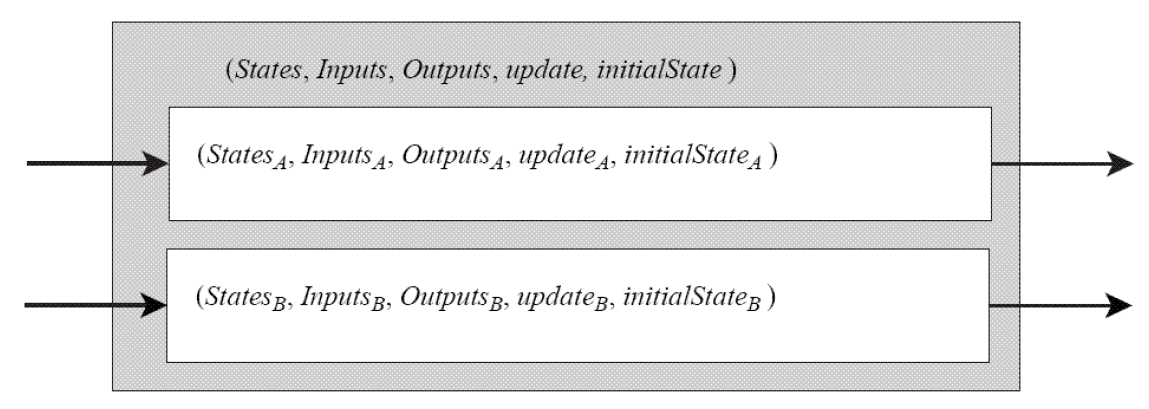
\includegraphics[scale=0.4]{img/sidebyside.png}
\caption{Esempio di composizione side-by-side}\label{fig:sidebyside}
\end{figure}
\paragraph{Composizione sincrona}
In questo caso gli stati reagiscono insieme, la macchina a stati che si ottiene è formata dalla composizione degli stati precedenti:
$$S_C=S_A \times S_B$$
La macchina a stati che si ottiene è mostrata in \figurename\,\ref{fig:sidesincrona} vediamo che due stati non sono raggiungibili in quanto non vi è alcun modo in cui gli ingressi possano arrivare a quel valore.
\begin{figure}
\centering
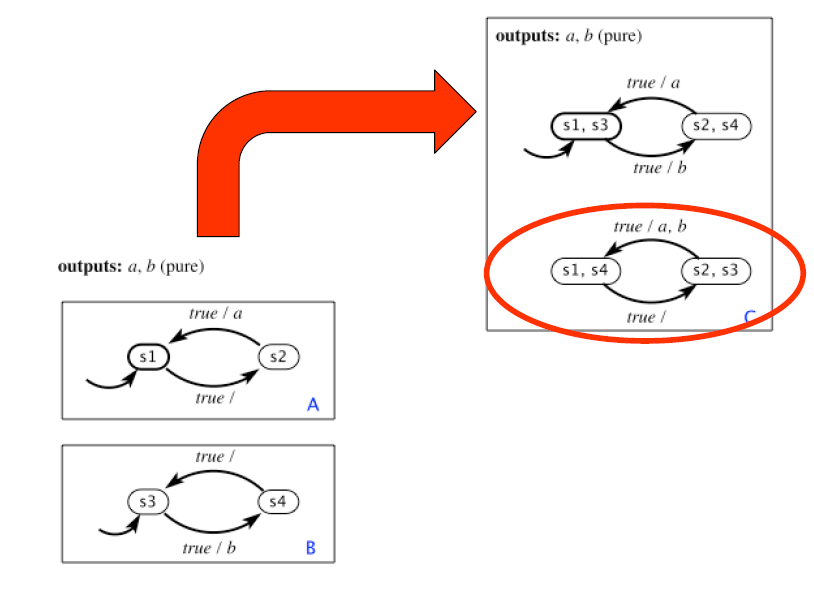
\includegraphics[scale=0.4]{img/sidesincrona.png}
\caption{Esempio di composizione side-by side sincrona}\label{fig:sidesincrona}
\end{figure}
Nel caso di composizione sincrona la nuova macchina che si viene a creare può essere espressa come:
$$
\begin{array}{lcl}
States & = & States_A \times States_B\\
Inputs & = & Inputs_A \times Inputs_B\\
Outputs & = & Outputs_A \times Outputs_B\\
initialState & = & initialState_A \times initialState_B\\
((S_A(n+1),S_B(n+1)),(o_A(n),o_B(n))) & = & update((S_A(n),S_B(n)),(i_A(n),i_B(n)))  
\end{array}
$$
dove 
$$
\begin{array}{rcl}
(S_A(n+1),o_A(n)) & = & update_A(S_A(n),i_A(n)) \mathtt{and} \\
(S_B(n+1),o_B(n)) & = & update_B(S_B(n),i_B(n)) 
\end{array}
$$
\paragraph{Composizione asincrona}
In questo caso gli stati reagiscono indipendentemente gli uni dagli altri, in questo caso tutti gli stati risultano raggiungibili come si vede dalla \figurename\,\ref{fig:sideasincrona} la composizione degli stati è eseguita tramite la semantica intervallata ed è il risultato di 
$$S_D=S_A\times S_B$$
\begin{figure}
\centering
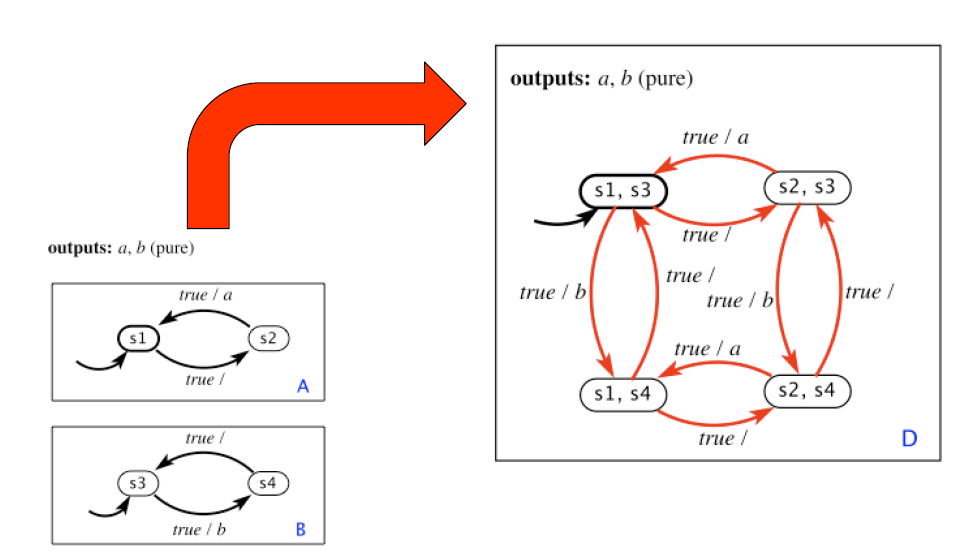
\includegraphics[scale=0.4]{img/sideasincrona.png}
\caption{Esempio di composizione side-by-side asincrona}\label{fig:sideasincrona}
\end{figure}
Nel caso invece di composizione asincrona la macchina a stati finita viene descritta da:
$$
\begin{array}{lcl}
States & = & States_A \times States_B\\
Inputs & = & Inputs_A \times Inputs_B\\
Outputs & = & Outputs_A \times Outputs_B\\
initialState & = & initialState_A \times initialState_B\\
((S_A(n+1),S_B(n+1)),(o_A(n),o_B(n))) & = & update((S_A(n),S_B(n)),(i_A(n),i_B(n)))  
\end{array}
$$
dove 
$$
\begin{array}{rcl}
(S_A(n+1),o_A(n)) & = & update_A(S_A(n),i_A(n)) \mathtt{and} S_B(n+1) = S_B(n) \& o_B = absent \mathtt{or}\\
(S_B(n+1),o_B(n)) & = & update_B(S_B(n),i_B(n)) \mathtt{and} S_A(n+1) = S_A(n) \& o_a = absent
\end{array}
$$
\subsubsection{Composizione in cascata}
La \emph{composizione in cascata} non è altro che il collegamento in serie di due macchine a stati come si vede dalla \figurename\,\ref{fig:cascade} dove l'output della prima macchina a stati è connesso all'input della seconda macchina. Anche in questo caso possiamo parlare di composizione sincrona e asincrona. 
\begin{figure}
\centering
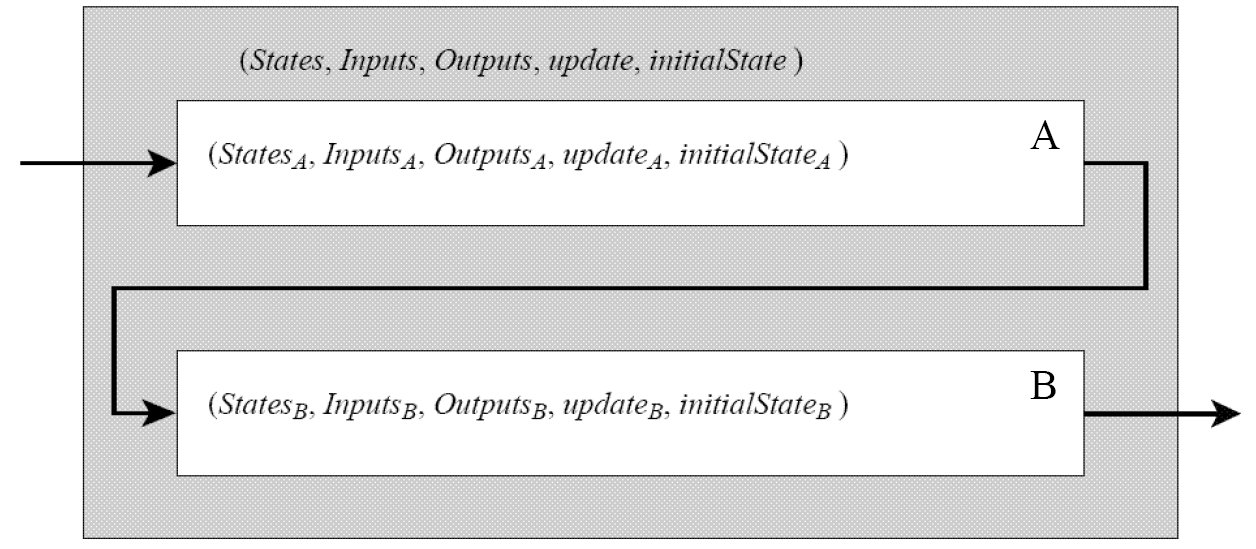
\includegraphics[scale=0.4]{img/cascade.png}
\caption{Esempio di composizione a cascata}\label{fig:cascade}
\end{figure}
Analizziamo ora un esempio di un semaforo nel quale una macchina a stati descrive il comportamento del semaforo utilizzato per le automobili \figurename\,\ref{fig:semaforoauto} mentre una seconda macchina a stati descrive il comportamento del semaforo pedonale \figurename\,\ref{fig:semaforoped}. 
\begin{figure}
\centering
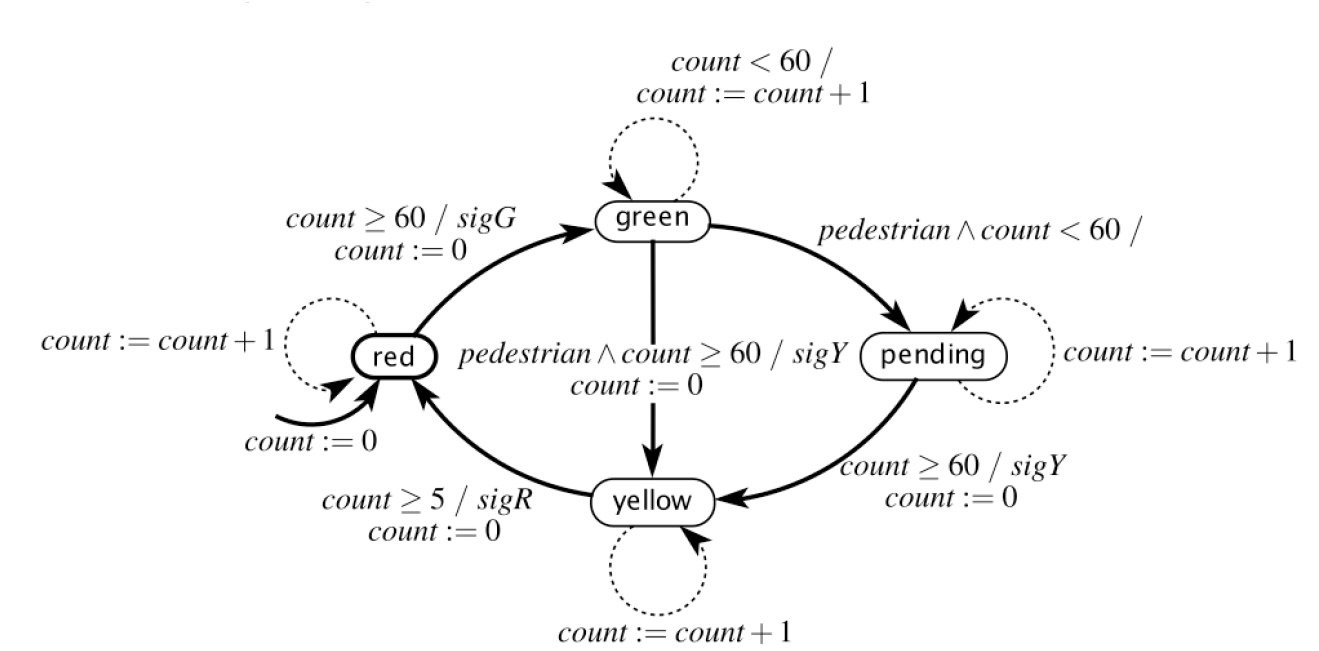
\includegraphics[scale=0.4]{img/semaforoauto.png}
\caption{FSM che modella il comportamento di un semaforo per le auto}\label{fig:semaforoauto}
\end{figure}
\begin{figure}
\centering
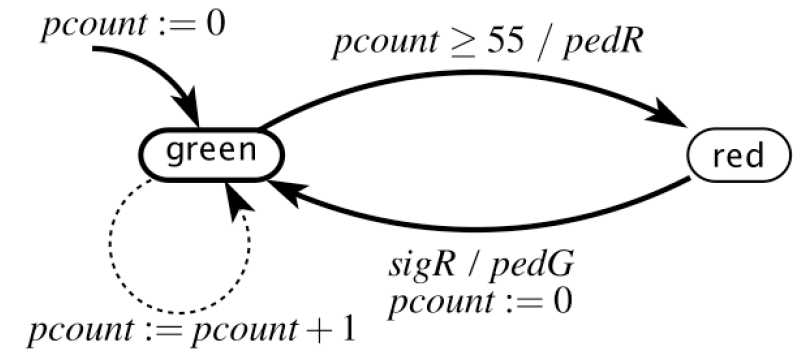
\includegraphics[scale=0.4]{img/semaforoped.png}
\caption{FSM che modella il comportamento di un semaforo per un attraversamento pedonale}\label{fig:semaforoped}
\end{figure}
In \figurename\,\ref{fig:semaforocomp} vediamo la composizione delle due macchine a stati finiti nella quale però sono stati rimossi gli stati non raggiungibili. In caso di composizione \emph{sincrona} la macchina reagisce simultaneamente nonostante sembra che esista una relazione causale tra le due. Ad esempio in questo caso sembrerebbe che la macchina agisca in modo sequenziale passando dal rosso al verde e viceversa ma bisogna tenere conto che in realtà gli stati che vengono raggiunti sono un insieme di stati e non vi è mai uno stato nel quale le due macchine non agiscono insieme.\\
\begin{figure}
\centering
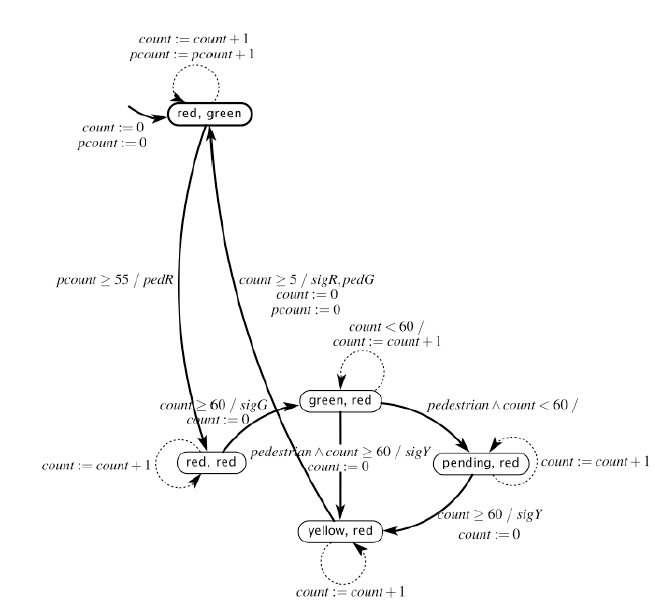
\includegraphics[scale=0.6]{img/semaforocomp.png}
\caption{Composizione in cascata delle due FSM precedenti}\label{fig:semaforocomp}
\end{figure}
Nel caso di composizione \emph{asincrona} invece le uscite di una macchina entrano negli ingressi dell'altra in modo indipendente dai cambiamenti delle macchine. Un esempio di composizione asincrona è mostrata in \figurename\,\ref{fig:cascadeasincrona}.\\
\begin{figure}
\centering
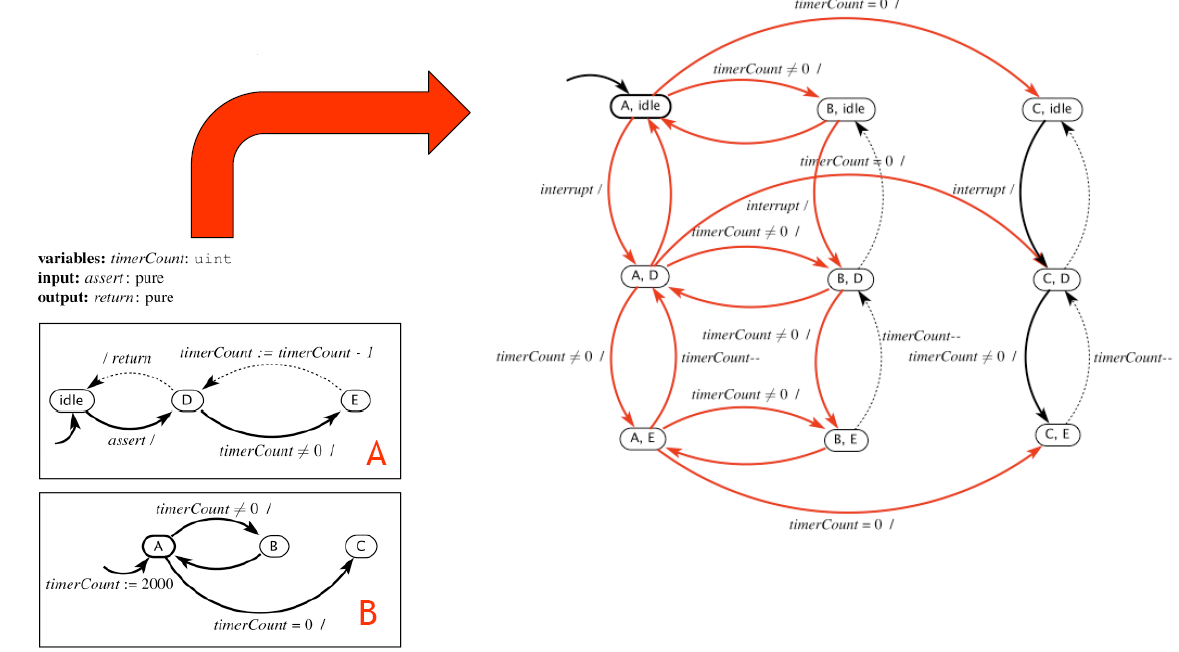
\includegraphics[scale=0.4]{img/cascadeasincrona.png}
\caption{Esempio di composizione in cascata asincrona}\label{fig:cascadeasincrona}
\end{figure}
\subsubsection{Composizione gerarchica}
Quando parliamo di composizione gerarchica facciamo riferimento ad un particolare tipo di FSM nella quale uno stato è rappresentato da una seconda FSM come nel caso di \figurename\,\ref{fig:gerarchica} in questo caso prima si raggiunge lo stato superiore e a quel punto si entra nello strato inferiore, nel caso entrambe le macchine producano un output questo non deve essere conflittuale.\\
\begin{figure}
\centering
\subfigure[]{
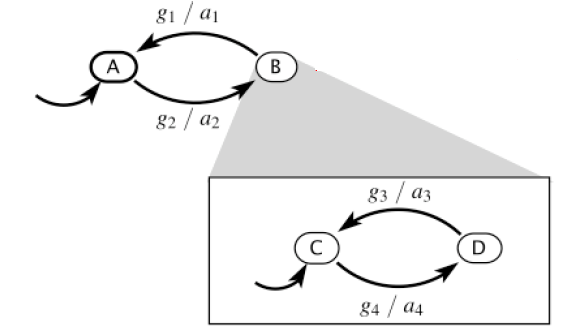
\includegraphics[scale=0.45]{img/gerarchia.png}
}
\subfigure[]{
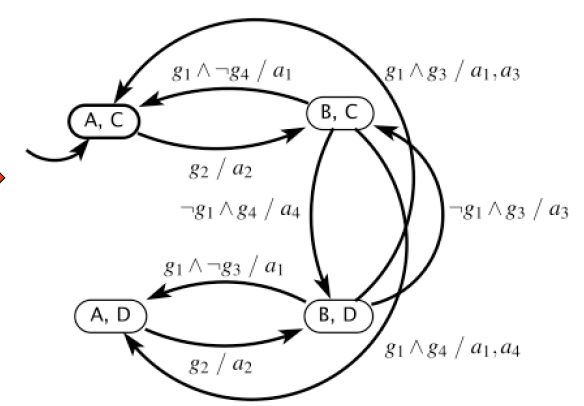
\includegraphics[scale=0.45]{img/gerarchiafsm.png}
}
\caption{Esempio di FSM gerarchica}\label{fig:gerarchica}
\end{figure}
A differenza degli altri casi il caso gerarchico permette diversi tipi di composizione. Ad esempio nel primo caso che analizziamo parliamo di \emph{memoria della transizione} ad esempio nella nostra macchina a stati quando raggiungiamo lo stato \emph{B} entriamo nella FSM composta dagli stati \emph{C} e \emph{D} a quel punto potremmo muoverci all'interno di quegli stati fino a quando non si presenti in ingresso il valore $g_1$ che ci fa tornare allo stato \emph{A}, nel caso di FSM con memoria una volta che torneremo nello stato \emph{B} ripartiremo dall'ultimo stato in cui abbiamo lasciato la macchina, un esempio delle transizioni è mostrato di seguito
$$A\xrightarrow{g_2/a_2}C\xrightarrow{g_4/a_4}D\xrightarrow{g_1/a_1}A\xrightarrow{g_2/a_2}D\xrightarrow{g_3\wedge g_1/a_3,a_1}A\dots$$
Esistono poi le FSM gerarchiche con rest come quella di \figurename\,\ref{fig:gerarchicareset} in questo caso la transizione che entra nello stato gerarchico è indicata da una freccia vuota. Il reset fa in modo che ad ogni ingresso in \emph{B} lo stato dal quale si parte sia sempre lo stato iniziale della sotto-FSM nel nostro esempio lo stato \emph{C}. Le transizioni in questo caso sono:
$$A\xrightarrow{g_2/a_2}C\xrightarrow{g_4/a_4}D\xrightarrow{g_1/a_1}A\xrightarrow{g_2/a_2}C\xrightarrow{g_4\wedge g_1/a_4,a_1}A\dots$$
\begin{figure}
\centering
\subfigure[]{
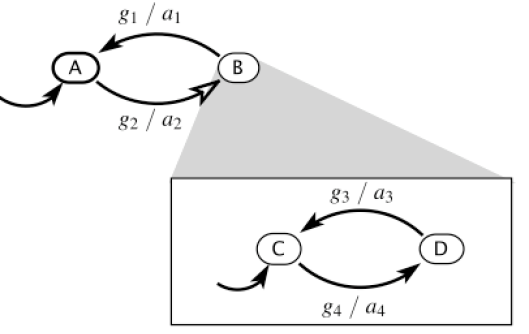
\includegraphics[scale=0.45]{img/gerarchiareset.png}
}
\subfigure[]{
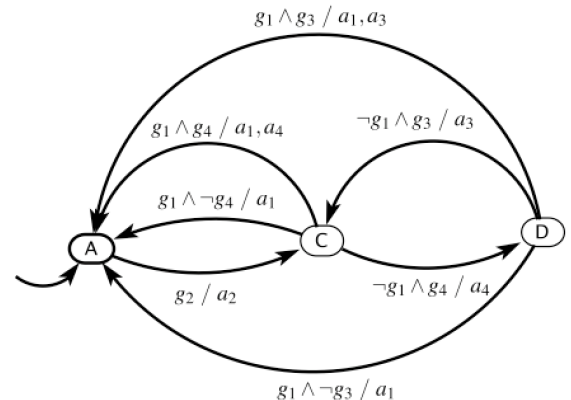
\includegraphics[scale=0.45]{img/gerarchiaresetfsm.png}
}
\caption{Esempio di FSM gerarchica con reset}\label{fig:gerarchicareset}
\end{figure}
L'ultima tipologia di composizione gerarchica è quella di \figurename\,\ref{fig:preemtiveger} ovvero una composizione gerarchica con \emph{preemtive}; il preemtive è un meccanismo per cui la valutazione della guardia che riporta la macchina nello stato \emph{A} è valutata prima di raggiungere lo stato corrente nella sottomacchina, nel caso la valutazione sia vera allora lo stato corrente non viene raggiunto.
\begin{figure}
\centering
\subfigure[]{
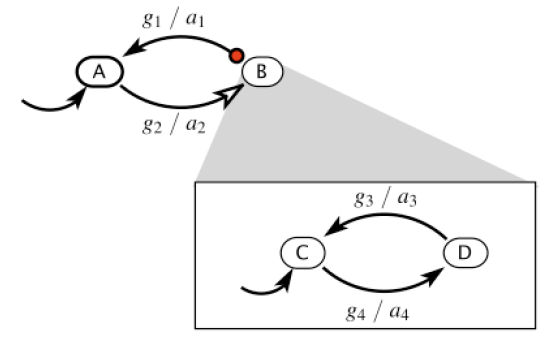
\includegraphics[scale=0.45]{img/preemtiveger.png}
}
\subfigure[]{
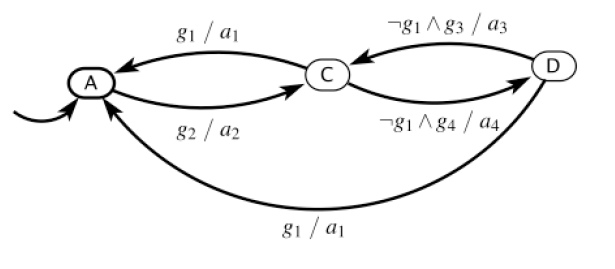
\includegraphics[scale=0.45]{img/preemtivegerfsm.png}
}
\caption{Esempio di FSM gerarchica con preemtive}\label{fig:preemtiveger}
\end{figure}
\subsection{Attori}
Gli attori non sono altro che dei componenti nei quali input e output sono esposti come in \figurename\,\ref{fig:attore} in questo caso però si tratta di modelli a tempo continuo, anche per gli  attori è possibile effettuare la composizione, la più comune è la composizione a \emph{feedback}.
\begin{figure}
\centering
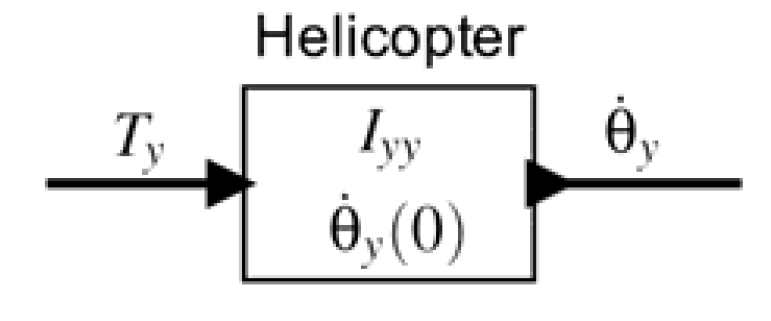
\includegraphics[scale=0.4]{img/attore.png}
\caption{Esempio di attore}\label{fig:attore}
\end{figure}
\subsection{Dataflow model}
$\dots$
\subsection{Multitasking}
Veramente volete ancora appunti sui \emph{pthread}?

%\section{Flusso di progetto nei sistemi eterogenei}\label{capitolo3}
Come abbiamo visto i sistemi embedded sono sistemi specializzati progettati per svolgere una o poche funzioni, molto spesso con vincoli stringenti. Questi tipi di sistemi sono progettati come \emph{SoC Multiprocessore} che sono diventati lo  standard di fatto di questo tipo di sistemi. Molti dei sistemi embedded hanno dei vincoli stringenti per quanto riguarda le prestazioni, l'ottimizzazione delle applicazioni per sistemi embedded complessi è un problema difficile, che richiede progettisti con un alto livello di esperienza per identificare la soluzione migliore.\\
Solitamente si utilizzano delle piattaforme hardware di base, tuttavia i vincoli stringenti richiedono processori dedicati per accelerare specifiche funzioni.\\
Per definire il problema dobbiamo considerare numerosi aspetti:
\begin{description}
\item[Job:] ovvero l'attività da eseguire e completare affinché il sistema soddisfi le specifiche.
\item[Punto di implementazione:] indica il modo nel quale svolgere un lavoro. Rappresenta una combinazione di \emph{latenza} e \emph{risorse necessarie}.
\item[Mapping:] assegna ogni \emph{job} ad un possibile \emph{punto di implementazione}, in modo da rispettare i vincoli imposti dalle risorse.
\item[Scheduling:] determina l'ordine di esecuzione di tutti i lavori.
\item[Obiettivo:] minimizzare il tempo di esecuzione complessivo dell'applicazione sull'architettura designata
\end{description}
Per quanto riguarda l'\emph{obiettivo} di minimizzare il tempo di esecuzione possiamo intervenire in diversi modi, come quello di analizzare, valutare ed ottimizzare differenti alternative, ed una volta individuata una soluzione valutarne la qualità prima della sua implementazione.\\
La progettazione di sistemi eterogenei a multi processore richiede diversi fasi:
\begin{itemize}
\item Una fase di partizionamento dell'applicazione (\emph{partitionig})
\item Una fase di assegnamento dei task ai diversi elementi architetturali (\emph{mapping})
\item La determinazione dell'ordine di esecuzione dei task (\emph{scheduling})
\end{itemize}
La parte di \emph{scheduling} e di \emph{mapping} è un problema \emph{NP-completo} inoltre il problema di un design e l'interfacciamento di componenti eterogenei può generare delle soluzioni non ammissibili.\\
Una rappresentazione imparziale e unificata di software ed hardware supporta la fase di progettazione ed analisi, permette una facile valutazione delle soluzioni individuate e inoltre permette la migrazione dei task tra la parte hardware e quella software. Tecniche di progettazione iterative permettono di valutare soluzioni differenti, aiuta a determinare l'implementazione migliore ed infine il partizionamento dei moduli permette un maching più preciso rispetto ai criteri di progettazione. Esistono inoltre dei metodi di parallelizzazione che possono valutare il grado di parallelismo a livello di :
\begin{itemize}
\item Istruzione
\item Dati 
\item Task
\end{itemize}
Tuttavia si introducono problemi di dipendenza che devono essere soddisfatti.\\
il parallelismo dei dati è definito come il parallelismo ottenuto dall'esecuzione concorrente che utilizza porzioni di dati differenti.
Il parallelismo dei task invece viene definito come il parallelismo ottenuto dalla computazione su diverse strutture dati.
In molti casi si utilizza un misto delle due tecniche soprattutto in ambito scientifico.\\
Un \emph{grafico dei task} è un grafico $G=(T,E)$ nei quali i nodi rappresentano un gruppo di istruzioni e gli archi rappresentano le dipendenze, solitamente gli archi vengono indicati con il quantitativo di dati da trasferire in modo da considerare anche il ritardo di comunicazione.
Nel caso di grafi ciclici adotteremo la rappresentazione \emph{gerarchica dei grafi} nei quali i nodi son suddivisi in tre classi:
\begin{description}
\item[semplici:] un task senza altri sotto task,
\item[composto:] quando un task ha altri sotto task associati,
\item[loop:] task che rappresentano un ciclo in cui il corpo è un sotto-grafo
\end{description}
I meccanismi utilizzati per l'analisi devo preservare il \emph{comportamento osservabile} del programma, ovvero, consumare i bytes in input, rispettare l'output e la terminazione del programma; tuttavia l'output può subire alcune variazioni come una differente precisione o operazioni associate in modo diverso ma il compilatore deve dimostrare che le trasformazioni preservano il comportamento in caso contrario le ottimizzazioni devono essere conservative.\\
\subsection{Analisi delle dipendenze}
Un linguaggio sequenziale presenta un ordinamento totale dei vari blocchi, tuttavia per mantenere il comportamento osservabile del programma è sufficiente un \emph{ordinamento parziale} ma questo ordinamento deve essere scoperto. Prendiamo come esempio il codice seguente:
\begin{verbatim}
float foo(a, b) {
    float t1 = sin (a);
    float t2 = cos (b);
    return t1/t2;
}
\end{verbatim}
In questo caso riordinando \emph{t1} e \emph{t2} il comportamento della funzione non cambia. L'ordinamento nel codice sorgente risulta essere pessimistico, un analisi delle dipendenze individua in modo più specifico un ordinamento parziale e questo da la libertà al compilatore di risistemare il codice. L'analisi però risulta in molti casi \emph{incompleta}, infatti, nel caso migliore risulta \emph{precisa} in quello peggiore, invece, tende ad essere molto \emph{conservativa} questo porta alla creazione di false dipendenze che possono essere rimosse soltanto migliorando l'analisi.\\
Vediamo ora quali sono le tipologie di dipendenza analizzando come prima la dipendenza dei dati, il codice di esempio mostra un tipico caso di dipendenza dei dati dove un'operazione utilizza il valore proveniente da un'operazione precedente, si può costruire anche un grafico delle dipendenze come quello in \figurename\,\ref{fig:datadep}.
\begin{verbatim}
P = ...;
Q = ...;
R = P + Q;
S = Q + 1;
\end{verbatim}
\begin{figure}
\centering
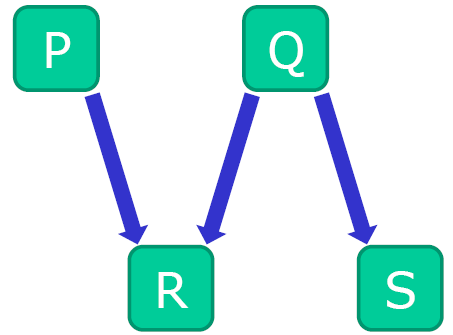
\includegraphics[scale=0.5]{img/datadep.png}
\caption{Esempio di grafico delle dipendenze sui dati}\label{fig:datadep}
\end{figure}
Esistono diverse categorie di dipendenze dei dati:
\begin{itemize}
\item Dipendenza \emph{flow} o anche \emph{Read After Write}
\item Dipendenza \emph{anti} o anche \emph{Write After Read}
\item Dipendenza \emph{output} o anche \emph{Write After Write}
\end{itemize}
Tuttavia le ultime due dipendenze sono tali a causa di riuso delle risorse e non sono vere dipendenze dei dati.\\
La seconda dipendenza che analiziamo è la \emph{dipendenza da controllo} in questo caso la dipendenza è dovuta al fatto che un'operazione può essere abilitata o disabilitata dall'esecuzione di un'altra istruzione come avviene nel caso di un costrutto \texttt{if}. In alcuni casi è possibile rimuovere alcune dipendenze come nell'esempio seguente:
\begin{verbatim}
if (P) {
    X = Y + 1;
    print(X);
}
\end{verbatim}
In questo caso è possibile eseguire l'istruzione che assegna il valore \emph{X} al di fuori dell'istruzione di controllo senza modificare il comportamento del programma.\\
L'analisi delle dipendenze tuttavia no è banale, un metodo come detto è quello che utilizza grafi delle dipendenze ma risulta di difficile computazione ed inoltre alcuni loop non sono esplicitati questo potrebbe portare a dipendenze non risolte. Un'altra metodologia è quella del \emph{task partitioning} nel quale di divide il problema assegnato in sottoproblemi come segue:
\begin{description}
\item[Obiettivi:] l'obiettivo primario viene suddiviso in \emph{n} sotto obbiettivi $O=\{o_1,o_2,\dots, o_n\}$ composti da 
\item[Blocchi:] o anche chiamati \emph{partizioni} $P=\{p_1,\dots, p_m$
\end{description}
queste partizioni devo rispettare alcune proprietà:
\begin{itemize}
\item $p_1 \cup p_2 \cup \dots \cup p_m = O$
\item $p_i\cap p_j = \emptyset \forall i\neq j$
\item la funzione di costo $c(P)$ deve essere minimizzata.
\end{itemize}
Tale funzione di costo esprime la qualità del sistema e può includere il \emph{costo del sistema}, la \emph{latenza} e il \emph{consumo di energia}.
Esistono diversi metodi per effettuare il partitioning del sistema anche se è difficile valutare il costo della soluzione, possiamo distinguere i metodi in due categorie, metodi \emph{esatti} che comprendono \emph{enumerazione} e \emph{integer linear programming} e metodi \emph{euristici} i quali possono essere \emph{costruttivi} come il \emph{random mapping} o il \emph{clustering gerarchico}, o metodi \emph{iterativi} del quale fanno parte il \emph{Kernighan-Lin Algorithm} e la \emph{simulated annealing}.
\paragraph{Linear Programming}
Questo metodo è un problema NP-completo, il tempo di esecuzione dipende esponenzialmente dalla dimensione del problema, tuttavia problemi con più di mille variabili vengono risolti con buoni risultati.
\paragraph{Random mapping}
Ogni oggetto viene assegnato in modo casuale ad un blocco, questo metodo è utilizzato per fornire un punto di partenza per i sistemi iterativi.
\paragraph{Clustering gerarchico}
Assumiamo una funzione di vicinanza e determiniamo quanto vogliamo che crescano due oggetti vicini, partiamo con un singolo blocco da questo calcoliamo la funzione di vicinanza degli altri blocchi, troviamo i due blocchi più vicini e li uniamo fino a quando non raggiungiamo i criteri di terminazione.
\subsection{Mapping e Scheduling}
Durante la fase di mapping e di scheduling consideriamo sia la parte di task sia la comunicazione. Lo scopo è quello di considerare diversi vincoli di progettazione per determinare delle soluzioni ammissibili come limiti di area o componenti sui quali non è possibile effettuare alcune operazioni. La comunicazione deve essere considerata per effettuare operazioni di ottimizzazione efficienti, inoltre, diverse implementazioni hardware possono portare a miglioramenti nelle performance.
Un esempio di queste ottimizzazione è la tecnica \emph{ant colony} nella quale si parte da una prima esecuzione del programma che aiuta ad individuare i punti critici, in una seconda fase si analizzano e si valutano le diverse combinazioni di mapping e di scheduling. Principi stocastici garantiscono la completa esplorazione. I vantaggi di questa tecnica è che è più veloce delle altre, per quanto possibile scarta le soluzioni che non soddisfano i requisiti ed inoltre esplora efficacemente anche circuiti di grosse dimensioni.
%\section{Performance estimation}\label{capitolo4}
Per verificare se un sistema rispetta o no le specifiche è necessario testare il sistema una volta realizzato. Esistono diversi meccanismi per effettuare questi test ma possiamo dividerli in due categorie, i metodi \emph{host profile} nei quali la strumentazione è eseguita su una macchina diversa da quella testata detta appunto \emph{host} e  metodi \emph{target profile} nei quali le informazioni vengono prelevate direttamente sulla piattaforma o so un prototipo. Le analisi di tipo \emph{target profile} sono utilizzate per misurare le performance di un sistema soprattutto quando alcune parti dell'applicazione sono realizzate tramite librerie proprietarie delle quali non se ne conosce l'efficienza, oppure nel caso in cui i valori di ingresso sono disponibili solo per la macchina target ma soprattutto nel caso in cui le tecniche di ottimizzazione richiedano un'analisi più accurata. In alcuni casi è anche possibile fare delle misurazioni anche su architetture incomplete, quando ad esempio l'architettura finale non è ancora disponibile oppure quando si vogliono testare più soluzioni per alcune parti del sistema.\\
Per effettuare le misurazioni sulla macchina target si sfruttano le librerie \emph{openMP}, in una prima fase il progettista inserisce i costrutti \emph{pragmas} nelle sezioni di codice che richiedono di essere misurati, successivamente questi costrutti vengono sostituiti da opportune istruzioni per la misurazione, nella fase di \emph{compilazione ed esecuzione} il codice viene compilato ed eseguito sull'architettura designata. Nella terza fase si collezionano tutti i dati e si confrontano con quelli già raccolti per stimare le performance dell'architettura finale. Un esempio di questo flusso è mostrato in \figurename\,\ref{fig:metodoflow}.\\
\begin{figure}
\centering
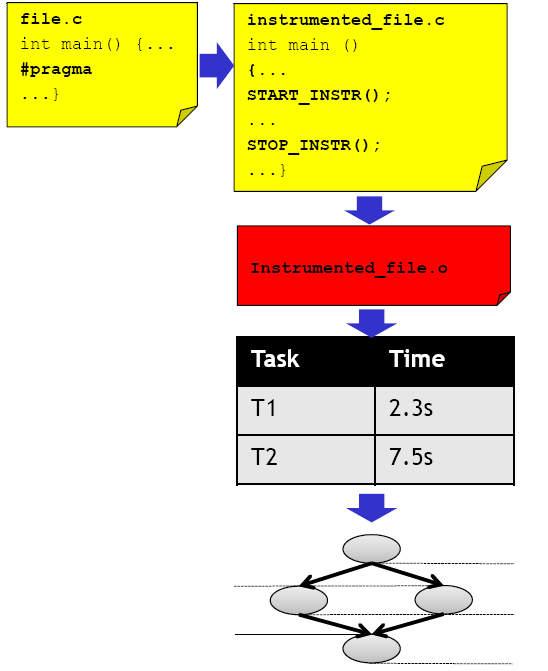
\includegraphics[scale=0.4]{img/metodoflow.png}
\caption{Flusso di raccolta dei dati}\label{fig:metodoflow}
\end{figure}
L'aggiunta delle istruzioni \emph{pragma} non influenza l'indipendenza del codice dall'architettura, è possibile tuttavia personalizzare il codice per una singola architettura tramite la definizione di un file di configurazione.\\
In alcuni casi l'analisi sull'architettura target non è fattibile, o perchè l'architettura non è ancora disponibile o perchè il progettista deve scegliere tra una vasta serie di elementi diversi. Sono state introdotte perciò delle metodologie per la creazione automatica di modelli per l'analisi delle performance i quali non richiedono alcuna conoscenza sull'architettura targhe, sfruttano il \emph{GCC Register Transfert Language} ma soprattutto permettono l'\emph{host profiling}. In \figurename\,\ref{fig:gccschema} vediamo come il compilatore esegue la trasformazione del codice sorgente in codice assembly.
\begin{figure}
\centering
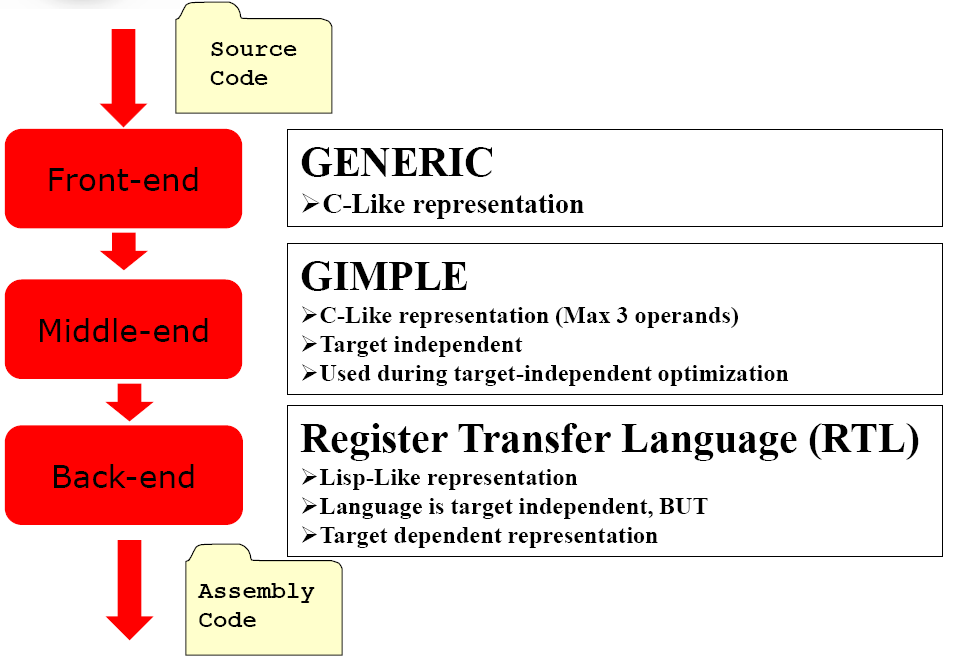
\includegraphics[scale=0.4]{img/gccschema.png}
\caption{Flusso di compilazione in GCC}\label{fig:gccschema}
\end{figure}
Il modello lineare è un'approssimazione del modello reale che non tiene in considerazione alcuni aspetti architetturali come il VLIW o la cache. I vantaggi di questo modello sono il fatto che esso è adattativo, semplice e leggibile e abbastanza accurato per essere usato per alcune fasi della progettazione.
Dati i modelli esistono diversi tipi di analisi che possono essere eseguite:
\begin{itemize}
\item \emph{Dinamica} che permette di tenere in considerazione come le performance dipendano dai dati 
\item \emph{RTL} che permette di considerare alcuni aspetti architetturali della macchina targhet
\item \emph{Sequenziale} permette di tenere in considerazione aspetti architetturali specifici come la pipeline, tuttavia questo tipo di analisi è estremamente difficile in quanto è difficile modellare gli effetti di tali aspetti.
\end{itemize}
Un simulatore o una piattaforma reale non è disponibile durante le fasi iniziali della progettazione dobbiamo costruire cosi un modello matematico per ogni singolo elemento. Tale procedimento richiede che il compilatore estragga dei dati per ogni elemento, tuttavia in alcuni casi alcuni processori utilizzano un loro compilatore proprietario che non permette di di estrarre rappresentazioni intermedie. Una soluzione allora è quella di approssimare la soluzione del compilatore proprietario a quella di GCC per fare ciò si utilizza una rappresentazione intermedia denominata \emph{GIMPLE} la quale è indipendente dall'architettura. Tuttavia il compilatore proprietario e GCC effettuano ottimizzazioni differenti.
\subsection{Task graph performance estimation}
Combinando i risultati delle precedenti analisi sui singoli task si cerca di stimare le performance globali, tuttavia l'esecuzione di alcuni task è correlata ad altri come nell'esempio di \figurename\,\ref{fig:taskgraph}
\begin{figure}
\centering
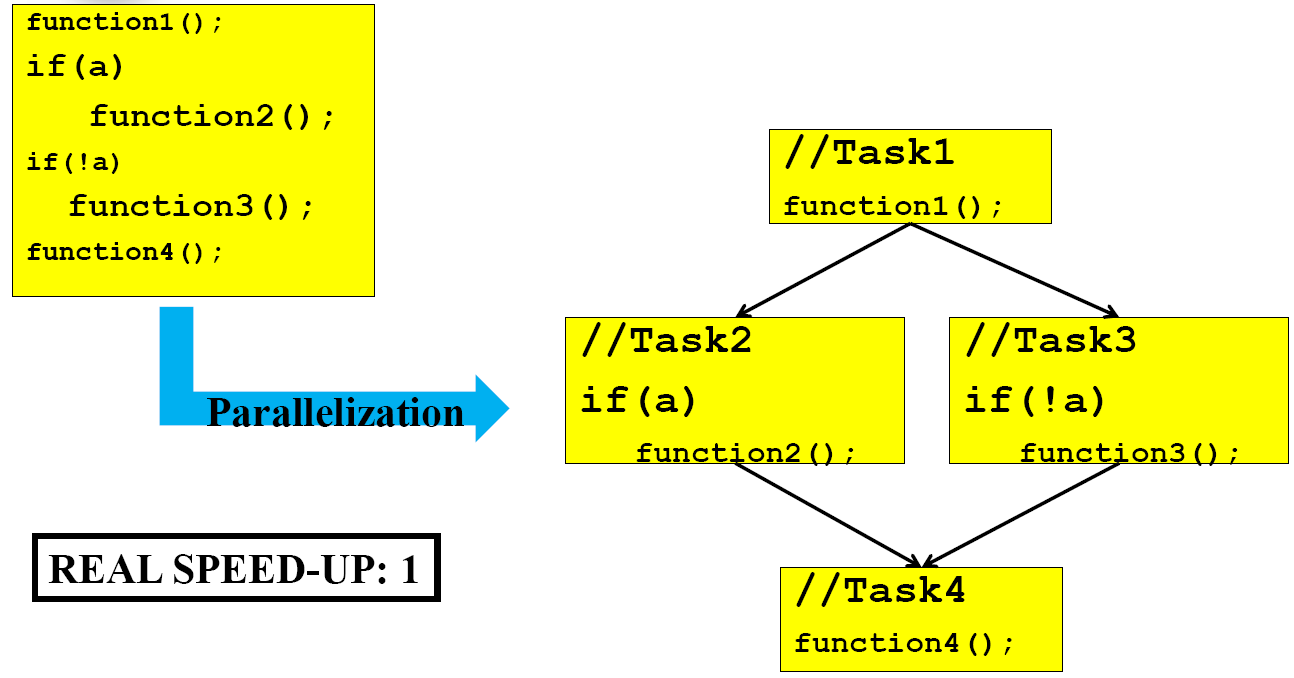
\includegraphics[scale=0.3]{img/taskgraph.png}
\caption{Esempio di grafico dei task}\label{fig:taskgraph}
\end{figure}
In questo metodo si tiene conto sia del percorso di esecuzione sia della topologia del task graph, il valore globale è dato dalle performance stimate moltiplicate per il loro peso sommate al contributo fornito da ogni percorso di esecuzione. Il contributo di ogni percorso è calcolato considerando le performace sul task graph quando solo il percorso di esecuzione è attivo. Il costo di creazione e distruzione dei task è costante. La frequenza dei diversi percorsi è ottenuta tramite profilazione dell'appllicazione tramite simulazione, ogni percorso è identificato da un intero, i percorsi possibili quelli che cominciano nel punto d'entrata e finiscono all'uscita della fnzione. Un esempio di tale meccanismo è mostrato in \figurename\,\ref{fig:taskestiamtion1} e \ref{fig:taskestiamtion2} dalla quale possiamo ricavare che:
$$\dfrac{(E_{p1}*F_{1})+(E_{p2}*F_{2})}{F_1+F_2}=\dfrac{(3000*0.2)+(3000*0.8)}{0.2+0.8}=3000$$
\begin{figure}
\centering
\subfigure[]{
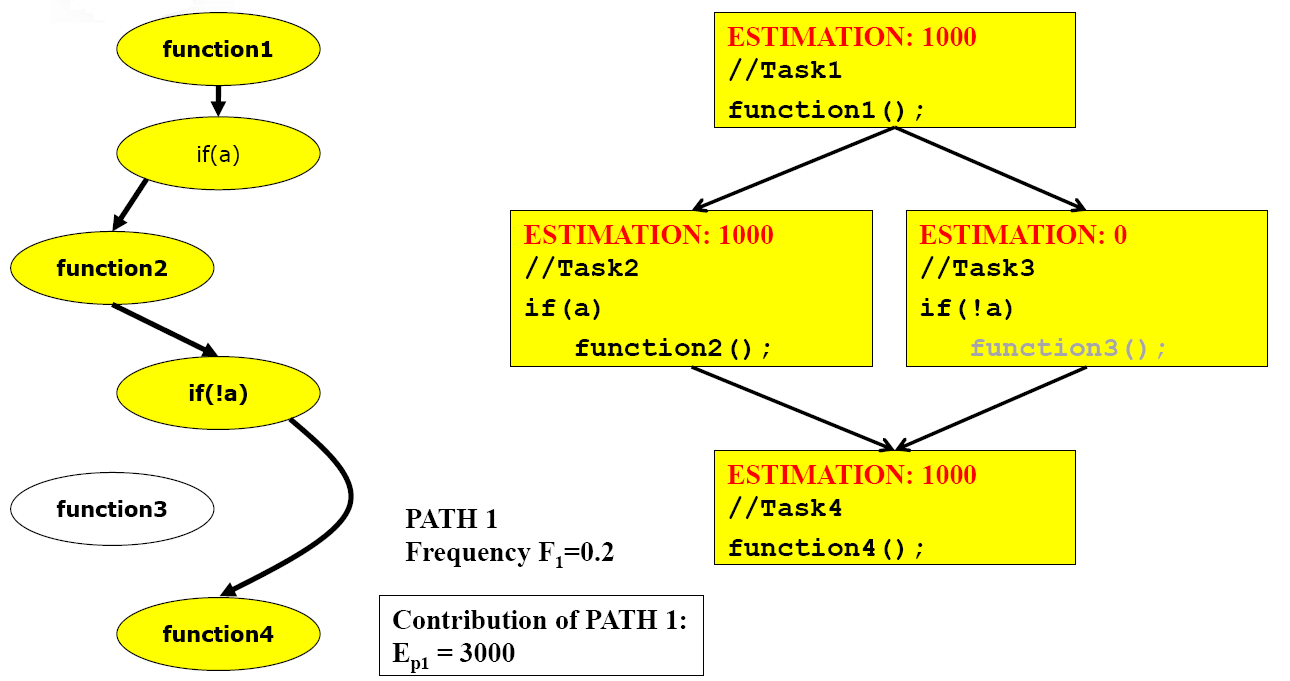
\includegraphics[scale=0.4]{img/taskestimation1.png}
\label{fig:taskestiamtion1}
}
\subfigure[]{
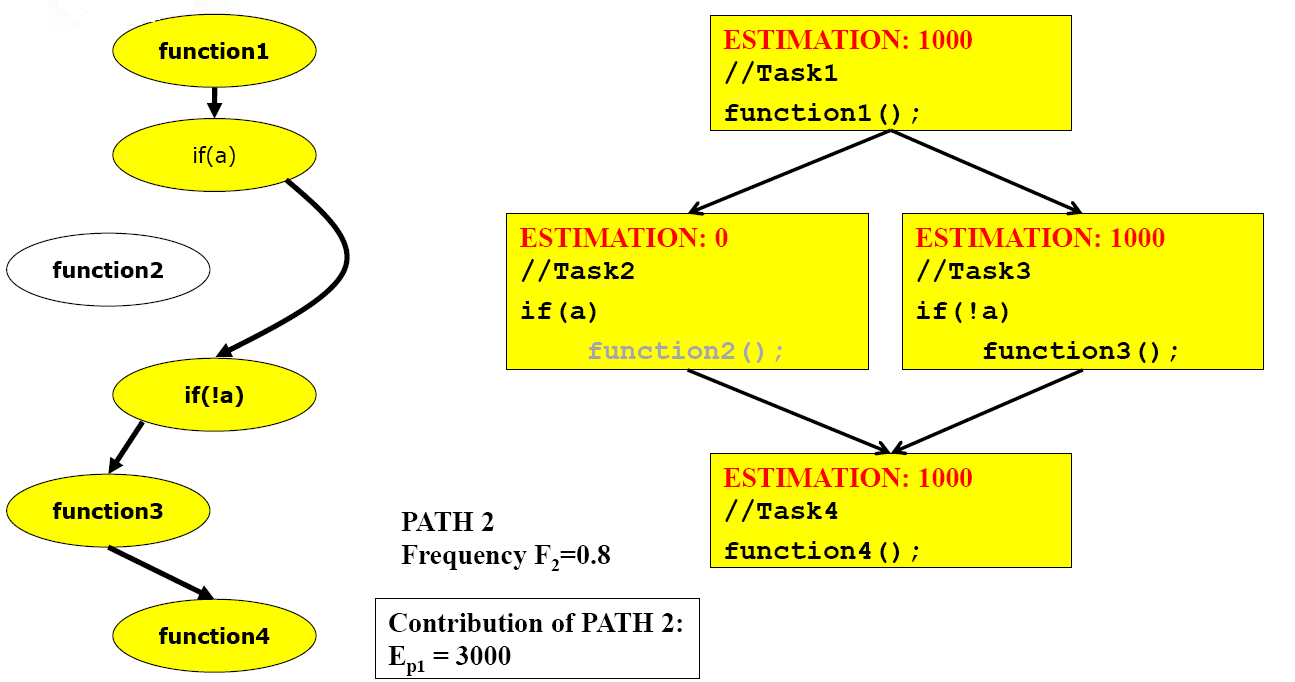
\includegraphics[scale=0.4]{img/taskestimation2.png}
\label{fig:taskestiamtion2}
}
\caption{Attivazione dei percorsi}
\end{figure}
%\section{Progettazione a basso consumo di potenza}\label{capitolo5}
Nel corso degli anni ci si è spostati verso la progettazione di sistemi hardware che consumassero sempre meno. Le motivazioni che hanno portato a questa evoluzione sono molteplici e di diversa natura; alcune di queste sono:
\begin{description}
\item[Tecnologiche:] l'aumento della frequenza e dei transistor presenti nel circuito obbligano ad un minor consumo di energia
\item[Commerciali:] la diffusione di dispositivi portatili che richiedono alte prestazioni e un basso consumo energetico
\item[Economiche:] ridurre il costo del \emph{packaging} del comparto batterie
\end{description}
La diffusione di dispositivi portatili ha portato ad avere un \emph{trade-off} tra le performance ed il consumo energetico.\\
Il design a basso consumo e le metodologie di stima del consumo di potenza devono essere valutate ad un diverso livello di astrazione durante tutto il processo di progettazione; i diversi livelli sono
\begin{itemize}
\item System Level
\item Behavioral Level
\item RT (Register Transfer) Level
\item Gate Level
\item Transistor Level
\end{itemize}
L'evoluzione attuale della tecnologia delle batterie è insufficiente rispetto all'evoluzione odierna dei circuiti, infatti, le capacità delle batterie aumentano all'incirca del 10\%-15\% all'anno mentre il consumo dei circuiti aumenta molto più velocemente, questo comporta un gap notevole tra il fabbisogno di potenza dei circuiti e la disponibilità data dai pacchi batterie.\\
Ad oggi la tecnologia più utilizzata per la realizzazione di circuiti digitali è quella \textbf{CMOS} in quanto la velocità di switching è notevole ed il consumo di corrente è intrinsecamente basso.
Il consumo di potenza nei CMOS è dato da 
$$P=P_{switching}+P_{short-circuit}+P_{leakage}$$
Dove $P_{switching}$ è la potenza necessaria per caricare e scaricare il condensatore durante il cambio di contesto del transistor $P_{short-circuit}$ è la corrente che va da $V_{dd}$ a $GND$ durante la transizione di uscita ed infine $P_{leakage}$ è la componente data dalla corrente di leakage.\\
La parte $P_{switching}$ è la parte predominante della dissipazione di potenza e l'obiettivo dei progettisti è quello di minimizzare questo fattore durante la fase di design del sistema. Per quanto riguarda, invece, $P_{short-circuit}$ e $P_{leakage}$ per minimizzarli occorre agire a livello tecnologico e non risulta essere una cosa semplice.\\
Vediamo ora come caratterizzare in modo più accurato la potenza di switching; distinguiamo inanzi tutto due casi:
\begin{itemize}
\item Transizione da $0 \rightarrow V_{dd}$ Fig. \ref{fig:vddoutput}
\item Transizione da $V_{dd} \rightarrow 0$ Fig. \ref{fig:ooutput}
\end{itemize}
\begin{figure}[hbt]
\begin{minipage}[b]{8cm}
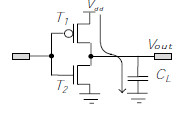
\includegraphics[width=7cm]{img/vddoutput.png}
\caption{Transizione $0 \rightarrow V_{dd}$}\label{fig:vddoutput}
\end{minipage}
\ \hspace{2mm} \hspace{3mm} \
\begin{minipage}[b]{8cm}
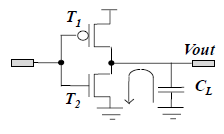
\includegraphics[width=7cm]{img/ooutput.png}
\caption{Transizione $V_{dd} \rightarrow 0$}\label{fig:ooutput}
\end{minipage}
\end{figure}
L'energia dissipata nel primo caso è data da:
\begin{itemize}
\item l'energia dissipata dal PMOS $T_1$ uguale a $\frac{1}{2}C_LV_{dd}^2$
\item l'energia immagazzinata in $C_L$ uguale a $\frac{1}{2}C_LV_{dd}^2$
\item l'energia derivante dalla carica uguale a $C_LV_{dd}^2$
\end{itemize}
Nel secondo caso abbiamo invece un'unica componente di dissipazione che è l'energia dissipata da $T_2$ uguale a $\frac{1}{2}C_LV_{dd}^2$.\\
Se le transizioni $0 \rightarrow V_{dd}$ e $V_{dd} \rightarrow 0$ avvenissero con la frequenza di clock $F_{CLK}$ avremo che la potenza dissipata dallo switching è data da 
$$P_{SW} = \frac{1}{2}C_LV_{dd}^2 f_{CLK}$$
Ma visto che ciò non accade e supponendo che $\alpha$ sia la probabilità che un gate commuti avremmo che la potenza media di switching dissipata da un CMOS è:
$$P_{SW} = \alpha \frac{1}{2}C_LV_{dd}^2 f_{CLK}$$
Definiamo ora la \emph{capacità effettiva} (o capacità di switching) un elemento che comprende il carico all'uscita del gate e la probabilità di switch.
$$C_{eff} = \alpha C_L$$
L'obbiettivo dei progettisti che cercano di minimizzare il consumo di potenza è quello di ridurre il più possibile $C_{eff}$ a qualsiasi livello di astrazione  e di scalare  $V_{dd}$ e $f_{CLK}$ i quali danno un risultato migliore in termini di efficienza ma che hanno anche un grande impatto in termini di performance.\\
La potenza dissipata per corto circuito si ha quando abbiamo un transizione nel valore di uscita; durante questa transizione abbiamo un percorso diretto tra $V_{dd}$ e $GND$.
Definendo $V_{ThN}$ e $V_{ThP}$ i rispettivi tensioni di soglia dell'NMOS e del PMOS ed essendo $V_{IN}$ la tensione di ingresso, se l'equazione seguente è soddisfatta:
$$V_{ThN} < V_{IN} < V_{dd} - |V_{ThP}| $$
Allora esiste un percorso tra $V_{dd}$ e $GND$ in quanto le transizioni dell'NMOS e del PMOS non sono simultanee.\\
Se definiamo $I_{SC}$ la corrente media di corto circuito otteniamo che la potenza media dissipata da questo caso è data da 
$$P_{SC} = I_{SC} V_{dd}$$
Questa componente è significativa solo nel caso il tempo di salita/discesa degli input è molto più grande dei tempi all'uscita. Se $V_{dd}$ soddisfa la seguente condizione:
$$V_{dd} < V_{ThN} + |V_{ThP}|$$
allora abbiamo che $I_{SC} = 0$ In quanto NMOS e PMOS non sono mai attivi simultaneamente.\\
Per quanto riguarda la potenza di leakage possiamo distinguere due componenti:
\begin{itemize}
\item Corrente di polarizzazione inversa del diodo attraverso il \emph{drain} del transistor: $I_L$
\item Correnti di sotto-soglia attraverso i canali a transistor spento: $I_{ds}$
\end{itemize}
La potenza di leakage dissipata dai gate del CMOS è data da:
$$P_{Leakage} = (I_L+ I_{ds}) V_{dd}$$
Questo valore è intorno al 5\% della potenza dissipata quando parliamo della tecnologia a 350nm mentre sale al 50\% nel caso di tecnologia a 90nm.\\
Il metodo migliore per risparmiare energia è minimizzare la capacità effettiva del circuito $C_{eff}$ definito come: $C_{eff} = \alpha C_L$; questa minimizzazione può essere effettuata a diversi livelli di astrazione. Sia minimizzando $C_L$
\begin{itemize}
\item Usando la logica CMOS dinamica
\item Usando la logica pass-gate
\item Dimensionando in maniera corretta transistor e interconnessioni
\item Ottimizzando al massimo i routing e i piazzamenti
\end{itemize}
sia minimizzando il fattore di switching $\alpha$ tramite:
\begin{itemize}
\item Ottimizzazioni basate si architetture parallele e di pipelined
\item Tecniche di encoding e di data rappresentation
\item Minimizzazione logica e tecnology mapping
\item Tecniche di shut-down basate sul clock gating
\end{itemize}
\subsection{Fattori di influenza di $C_{eff}$}
Esistono diversi fattori che influenzano il $C_{eff}$ e li analizzeremo uno per uno con degli esempi
\paragraph{Logic Function} Prendiamo un NOR a 2-input $A$ e $B$ implementati tramite tecnologia CMOS.
Assumiamo che $A$ e $B$ siano indipendenti ed equiprobabili ovvero 
$$p(A = 1)=p(B = 1)=\frac{1}{2}$$
ed che si abbia una sola transizione per ciclo di clock.
La probabilità che l'output sia uguale a 1 è:
$$p(O = 1)= (1-p(A = 1))(1-p(B = 1)) = \frac{1}{4}$$
mentre la probabilità che l'output sia uguale a 0 è:
$$p(O = 0) = 1- p(O = 1) = \frac{3}{4}$$
Costruiamo ora il diagramma della transizioni della porta NOR:
\begin{figure}
\centering
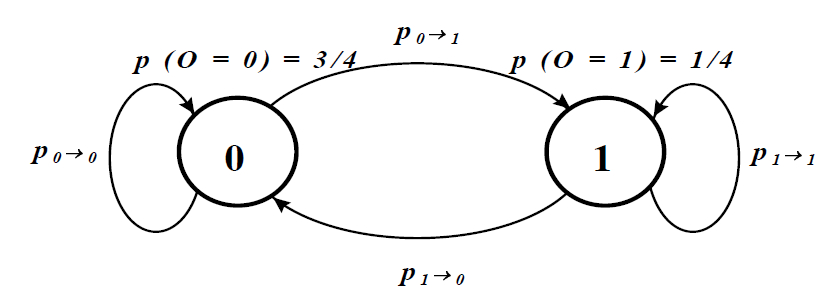
\includegraphics[width=10cm]{img/logicFSM.png}
\caption{Diagramma delle transizioni della porta NOR}\label{fig:logicFSM}
\end{figure}
Per l'output O la probabilità di transizione $p_{0\rightarrow1}$ è data dalla probabilità che lo stato corrente sia 0 e che il prossimo stato sia 1:
$$p_{0\rightarrow 1}= p(O = 0)p(O = 1)= \frac{3}{4}\times\frac{1}{4} = \frac{3}{16}$$
Così valido per gli altri stati:
$$p_{1\rightarrow 0}= p(O = 1)p(O = 0)= \frac{1}{4}\times\frac{3}{4} = \frac{3}{16}$$
$$p_{0\rightarrow 0}= p(O = 0)p(O = 0)= \frac{3}{4}\times\frac{3}{4} = \frac{9}{16}$$
$$p_{1\rightarrow 1}= p(O = 1)p(O = 1)= \frac{1}{4}\times\frac{1}{4} = \frac{1}{16}$$
Arriviamo al fattore di switching che è uguale a:
$$\alpha = p_{0\rightarrow 1} + p_{1\rightarrow 0} = \frac{3}{8}$$
\paragraph{Tecnologie}
La scelta nelle tecnologie CMOS può ricadere o in quella statica o in quella dinamica.
Nel caso di \emph{static CMOS} abbiamo che $C_L$è caricata a $V_{dd}$ ogni volta che è richiesta una transizione $0 \rightarrow 1$ all'uscita del transistor ed è scaricato a 0 ogni qualvolta vi è una transizione $1 \rightarrow 0$.\\
Nel caso di \emph{dynamic CMOS} $C_L$ è precaricato a $V_dd$ ad ogni ciclo di clock e scaricato a zero ogni qualvolta avviene una transizione $1 \rightarrow 0$. Come conseguenza di questo comportamento abbiamo che:
$$\alpha(dynamic \ CMOS) \geq \alpha(static \ CMOS)$$
e la capacità di solito è uguale a 
$$C_L(dynamic \ CMOS) \leq C_L(static \ CMOS)$$
Nel caso di static CMOS la probabilità di transizione dipende sia dalla probabilità di input sia dallo stato precedente; nel caso di dynamic CMOS invece la probabilità di switch dipende solo dalla probabilità degli ingressi.
Nel caso di static CMOS se gli input non cambiano dal ciclo di clock precedente allora le uscite non cambiano, nel caso dinamico invece gli output possono cambiare anche se gli input non cambiano.
\paragraph{Probabilità degli input}
Prendiamo il caso di una porta NOR a due ingressi implementata tramite tecnologia CMOS statica e assumiamo che gli input siano equiprobabili.
La probabilità che l'output sia uguale a 1 è data da:
$$p(O = 1) = (1-p(A = 1))(1-p(B = 1))$$
La probabilità che l'output sia 0 è data da:
$$p(O = 0) = 1 - p(O = 1)$$
La probabilità di una transizione da $0 \rightarrow 1$ è:
$$p_{0 \rightarrow 1} = p (O = 0)p(O = 1)=
(1-(1-p(A = 1))(1-p(B = 1)))(1-p(A = 1))(1 - p(B = 1))$$
\begin{figure}[hbt]
\centering
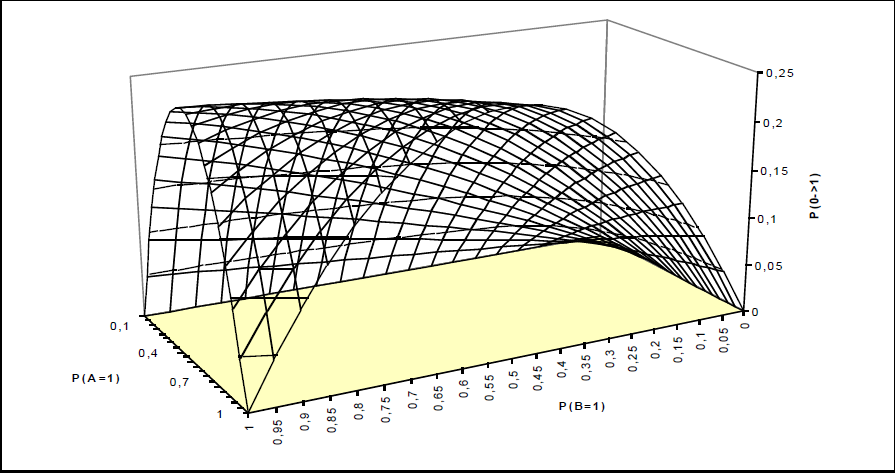
\includegraphics[scale=0.7]{img/p01.png}
\caption{Probabilità di transizione $0 \rightarrow 1$}
\end{figure}
\paragraph{Topologia del circuito} La topologia del circuito ha un forte impatto sulle attività di switching del circuito. Prendiamo ad esempio l'esempio di due implementazioni di un AND a 4 input. 
$$(1-(1-p(A = 1))(1-p(B = 1)))(1-p(A = 1))(1 - p(B = 1))$$
\begin{figure}[hbt]
\centering
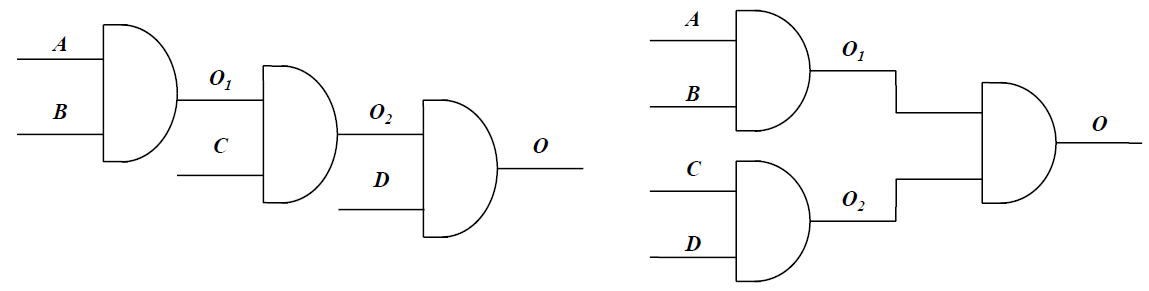
\includegraphics[scale=0.4]{img/and4input.png}
\caption{Due implementazioni di AND}
\end{figure}
Assumiamo che A,B,C,D sono indipendenti ed equiprobabili:
$$p(A = 1) = p(B = 1) = p(C = 1) = p(D = 1) = \frac{1}{2}$$
La probabilità che l'output di un AND con due ingressi sia uguale a 1 è data da:
$$p(O = 1) = p(A = 1)p(B = 1) = \frac{1}{4}$$
La probabilità che l'uscita della stessa porta sia uguale a 0 è uguale a:
$$p(O = 0) = 1-p(O = 1) = \frac{3}{4}$$
La probabilità di transizione $0 \rightarrow 1$ è data da:
$$p_{0\rightarrow 1}= p(O=0)p(O=1)§=\frac{3}{4}\frac{1}{4}=\frac{3}{16}$$
E il fattore di scambio è:
$$\alpha = p_{0\rightarrow 1} + p_{1\rightarrow 0} = \frac{3}{8}$$
Come vediamo dalla tabella in figura \ref{fig:2ANDimp}
\begin{figure}[hbt]
\centering
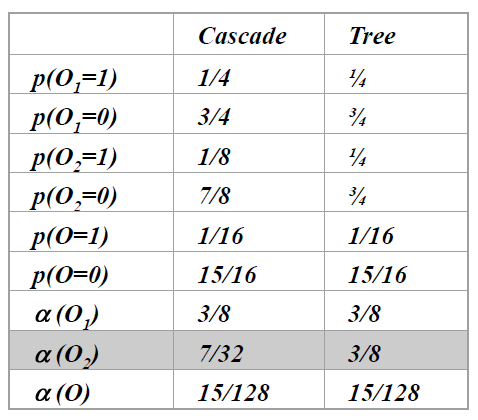
\includegraphics[scale=0.5]{img/2ANDimp.png}
\caption{Valori di comparazione per le due implementazioni di AND}\label{fig:2ANDimp}
\end{figure}
abbiamo che a parità di input la soluzione in cascata ha un fattore di switch minore.
Questo però analizzando solo i componenti statici e trascurando gli effetti di glitch che si hanno con l'analisi temporale.
\subsection{Voltage Scaling}
La velocità del circuito decresce tanto più $V_{dd}$ si avvicina a $V_{Th}$; usando una approssimazione del primo ordine possiamo modellizzare il ritardo $T_d$ del gate come:
$$T_d = \frac{C_{out}V_{dd}}{I}=\frac{C_{out}V_{dd}}{\eta(W/L)(V_{dd}-V_t)^2}$$
dove il fattore $\eta$ dipende dalla tecnologia e $W$ ed $L$ sono rispettivamente larghezza e lunghezza del canale CMOS.
L'obiettivo dei progettisti è quello di operare alla più bassa velocità possibile che permette la maggiore $V_{dd}$
Per ridurre la potenza preservando la velocità del circuito e il throughput computazionale dobbiamo ridurre l'incremento di ritardo dovuto al ridimensionamento del $V_{dd}$; esistono due approcci, il primo è quello di scalare in maniera proporzionale anche la tensione di soglia (Figura \ref{fig:thvdd}), oppure agendo sull'architettura implementando la parallelizzazione e la pipelining.
\begin{figure}[hbt]
\centering
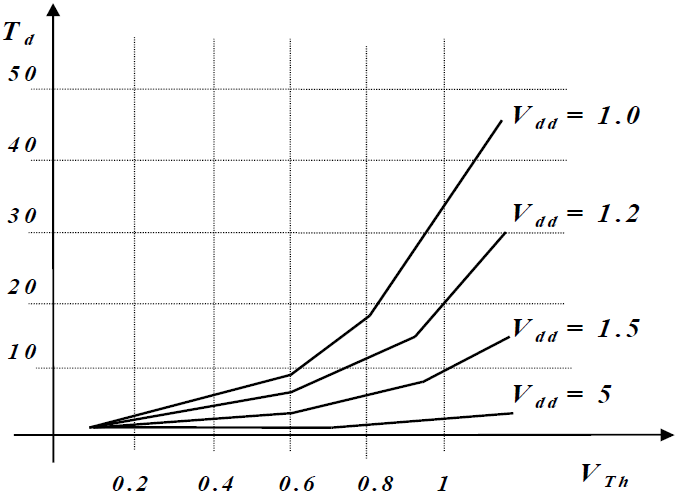
\includegraphics[scale=0.5]{img/thvdd.png}
\caption{Grafico dei ritardi in funzione di $V_{dd}$ e della tensione di soglia}\label{fig:thvdd}
\end{figure}
La riduzione della tensione di soglia permette di ridurre la potenza di switching senza perdere in velocità. I limiti sono dovuti al margine di rumore e all'incremento della corrente di sotto-strato $I_{DS}$; bisogna perciò trovare il giusto valore di bilanciamento tra la $P_{SW}$ che diminuisce al diminuire di $V_{Th}$ e $P_{Leakage}$ che invece aumenta al diminuire di $V_{Th}$
Nel caso invece di ottimizzazione dell'architettura si migliora il circuito in modo da renderlo più veloce, si riduce in seguito la $V_{dd}$ fino a ripristinare la velocità originale e si ha come effetto secondario la riduzione del consumo di energia. Come conseguenza però si ha un aumento della circuiteria che potrebbe aumentarne il consumo e parallelismo e pipelining hanno spesso un costo non indifferente.
\subsection{Tecniche di progetto a livello logico}
Analizziamo ora alcune tecniche di minimizzazione della potenza dissipata che si applicano alla progettazione a livello logico del circuito.
\subsubsection{Codifica degli stati}
Nel caso di sistemi orientati al controllo la specifica iniziale di una Macchina a Stati Finiti (FSM) è descritta tramite il Grafo di Transizione degli Stati (STG).
Il problema della codifica degli stati è quello di trovare un assegnamento di codici binari per gli stati in modo da minimizzare una determinata funzione di costo come ad esempio la potenza dissipata. Il problema è che l'assegnamento degli stati è un problema NP-completo.
Definiamo ora in modo più completo il problema della definizione degli stati; dati un STG assegnare dei codici binari agli stati in modo da minimizzare una data funzione di costo. In generale la funzione di costo C deve tener conto della distanza di \emph{Hamming} $H(s_i,s_j)$ tra i codici binari corrispondenti agli stati $s_i$ ed $s_j$ tra i quali può avvenire una transizione di stato. Una possibile funzione di costo può essere:
$$C=\sum H(s_i,s_j)$$
Una funzione di costo più accurata dovrebbe considerare altri fattori come la probabilità di transizione di stato. Come nel caso di un STG pesato i cui pesi rappresentano la probabilità di transizioni da uno stato $s_i$ ad uno $s_j$. L'idea è quello di assegnare codici \emph{vicini} a stati connessi da archi con i pesi più alti; la nuova funzione di costo diventa:
$$C = \sum W_{ij} H(s_i,s_j)$$
dove $W_{ij}$ è il peso assegnato all'arco che connette gli stati $s_i$ e $s_j$
\subsubsection{Tecniche di retiming}
La posizioni dei registri nel circuito sequenziale può impattare fortemente sull'area del circuito e di conseguenza anche sulle prestazioni e sulla potenza dissipata dal circuito. L'osservazione di base è che in un circuito sequenziale sincrono con un segnale di clock primario le uscite dei registri possono avere al più una transizione per ogni ciclo di clock. Questo riduce il numero di glitch o transizione spurie.
Le tecniche di \emph{Retiming} si basano sulla selezione di un insieme di porte logiche del circuito nei quali porre dei registri che minimizzano l'attività di transizione globale del circuito.\\
L'algoritmo è molto semplice basta selezionare un insieme di porte logiche caratterizzate da un elevato numero di glitch sulle uscite e un'alta probabilità che tali glitch si propaghino ai nodi successivi; all'uscita di queste porte si aggiunge un registro, nel caso dei registri siano già presenti nel circuito si spostano tali registri in modo da modificare la temporizzazione del circuito diminuendo la potenza dissipata ma senza impattare sulle funzionalità del circuito.
\subsubsection{Tecniche di pre-calcolo}
Sistemi digitali complessi hanno porzioni di logica che non eseguono calcoli utili  ad ogni ciclo di clock. L'idea base è quella di spegnere tale logica con l'obiettivo di limitare il consumo di potenza (\emph{logic shutdown}).\\
Nel caso del pre-calcolo si tratta di duplicare parti della logica con l'obiettivo di pre-calcolare i valori di uscita di una logica con cicli di clock in anticipo ed usare questi valori per ridurre l'attività di commutazione globale della logica durante i cicli di clock successivi.
Questo permette di spegnere la logica originale con un ciclo di anticipo. Questa tecnica però deve essere tenuta sotto controllo affinché la logica di precalcolo non diventi eccessiva.
\subsubsection{Tecniche di Clock Gating}
Le tecniche di clock gating consistono nel fermare selettivamente il segnale di clock del ciclo successivo in parti della logica dove non vengono svolti calcoli utili alla funzionalità globale del circuito.
Il segnale di clock viene disabilitato in corrispondenza di condizioni di riposo del circuito sequenziale, queste condizioni sono determinate a priori dal progettista.

\end{document}